\documentclass[11pt, oneside]{article}   	% use "amsart" instead of "article" for AMSLaTeX format
\usepackage[margin=1in]{geometry}                		% See geometry.pdf to learn the layout options. There are lots.
\geometry{letterpaper}                   		% ... or a4paper or a5paper or ... 
\usepackage{graphicx}				% Use pdf, png, jpg, or eps§ with pdflatex; use eps in DVI mode
								% TeX will automatically convert eps --> pdf in pdflatex		
\usepackage{amssymb}
\usepackage{xcolor}
\usepackage{makecell}
%SetFonts

%SetFonts


\newcommand{\diru}{$\uparrow$}
\newcommand{\dirl}{$\leftarrow$}
\newcommand{\dird}{$\nwarrow$}
\newcommand{\dirdl}{$\nwarrow\leftarrow$}
\newcommand{\dirdu}{$\nwarrow\uparrow$}
\newcommand{\dirlu}{$\leftarrow\uparrow$}
\newcommand{\dirdlu}{$\nwarrow\leftarrow\uparrow$}

\newcommand{\dirui}{\rotatebox[origin=c]{90}{$\Rsh$}}
\newcommand{\dirdi}{\rotatebox[origin=c]{90}{$\Lsh$}}
\newcommand{\diruui}{\rotatebox[origin=c]{90}{$\Rsh$}}
\newcommand{\dirdui}{$\nwarrow$\rotatebox[origin=c]{90}{$\Rsh$}}
\newcommand{\dirlui}{$\leftarrow$\rotatebox[origin=c]{90}{$\Rsh$}}
\newcommand{\dirldi}{$\leftarrow$\rotatebox[origin=c]{90}{$\Lsh$}}
\newcommand{\dirddi}{$\nwarrow$\rotatebox[origin=c]{90}{$\Lsh$}}
\newcommand{\dirudi}{$\uparrow$\rotatebox[origin=c]{90}{$\Lsh$}}
\newcommand{\dirdiui}{\rotatebox[origin=c]{90}{$\Lsh\Rsh$}}

\newcommand{\neginf}{$-\infty$}

\title{Midterm Practice Exam}
\author{Spring 2021}
%\date{17 October 2019}							% Activate to display a given date or no date

\begin{document}
\maketitle
\begin{enumerate}
\item Given the table below which was created using the Smith-Waterman algorithm for local alignment, (a) identify the local alignment score, and (b) perform trace-back to find the optimal alignment. 

{\footnotesize
\begin{tabular}{|c||c|c|c|c|c|c|c|c|c|c|}

\hline
& & \texttt{T} &  \texttt{T} &  \texttt{A} &  \texttt{C} &  \texttt{T} &  \texttt{G} &  \texttt{T} &  \texttt{G} &  \texttt{T} \\
\hline
\hline
&  0 &	 0 &	0 &	0 &	0 &	0 &	0 &	0 &	0 &	0 \\
\hline
\texttt{C} &  0 &	0  &	0 &	0 &	\dird 5 &	\dirl 4.5 &		\dirl 4 &	\dirl 3.5 &		\dirl 3 &	\dirl 2.5 \\
\hline 
\texttt{A} &  0 & 0 & 0 &  \dird 5 & \dirlu 4.5 &		\dirdlu 4 &	\dirdlu 3.5 &		\dirdlu 3 &	\dirdlu 2.5 &		\dirdlu 2 \\
\hline
\texttt{C} &  0 & 0 & 0 & \diru 4.5 &  \dird 10 & \dirl 9.5 & \dirl 9 & \dirl 8.5 & \dirl 8 & \dirl 7.5 \\
\hline 
\texttt{C} &  0 & 0 & 0 & \diru 4 & \dirdu 9.5 & \dirdlu 9 & \dirdlu 8.5 & \dirdlu 8 & \dirdlu 7.5 & \dirdlu 7 \\
\hline 
\texttt{C} & 0 & 0 & 0 & \diru 3.5 &  \dirdu 9 & \dirdlu 8.5 & \dirdlu 8 & \dirdlu 7.5 & \dirdlu 7 & \dirdlu 6.5 \\
\hline 
\texttt{C} &  0 & 0 & 0 & \diru 3 &   \dirdu 8.5 & \dirdlu 8 & \dirdlu 7.5 & \dirdlu 7 & \dirdlu 6.5 & \dirdlu 6 \\
\hline  
\texttt{T} &  0 & \dird 5 & \dird 5 & \dirl 4.5 & \diru 7.5 & \dird 13.5 & \dirl 13 & \dirdl 12.5 & \dirl 12 & \dirdl 11.5  \\
\hline 
\texttt{G} &  0 & \diru 4.5 & \diru 4.5 & \dirdlu 4 & \diru 7 & \diru 13 &  \dird 18.5 & \dirl 18 & \dirdl 17.5 & \dirl 17 \\
\hline 
\texttt{T} &  0 & \dird 5 & \dird 9.5 & \dirl 9 & \dirl 8.5 & \diru 12.5 & \diru 18 &  \dird 23.5 & \dirl 23 & \dirdl 22.5 \\
\hline 
\texttt{G} &  0 & \diru 4.5 & \diru 9 & \dirdlu 8.5 & \dirdlu 8 & \diru 12 & \dirdu 17.5 & \diru 23 &  \dird 28.5 &  \dirl 28 \\
\hline 
\end{tabular}
}

Optimal Local Alignment Score: \\[3em]
Optimal Local Alignment (note not all of the spaced will be used)\\
{
\Huge
\begin{tabular}{|c|c|c|c|c|c|c|c|c|c|c|c|c|c|c|c|c|c|c|}
\hline
~ & ~ & ~ & ~ & ~ & ~ & ~ & ~ & ~ & ~ & ~ & ~ & ~ & ~ & ~ & ~ & ~ & ~ & ~ \\
\hline
~ & ~ & ~ & ~ & ~ & ~ & ~ & ~ & ~ & ~ & ~ & ~ & ~ & ~ & ~ & ~ & ~ & ~ & ~ \\
\hline 
\end{tabular}
}
%%%%%%%%%%%%%%%%%%%%%%%%%
\clearpage
\item Given the Needleman-Wunsch table below, find the optimal global alignment for the two sequences. 

{\footnotesize
\begin{tabular}{|c||c|c|c|c|c|c|c|c|c|c|c|c|}

\hline
& & \texttt{T} &  \texttt{T} &  \texttt{A} &  \texttt{C} &  \texttt{T} &  \texttt{G} &  \texttt{T} &  \texttt{G} &  \texttt{T}\\
\hline
\hline
&  0 &	  \dirl -0.5 &	 \dirl  -1 &	\dirl -1.5 &	\dirl -2 &	\dirl -2.5 &	\dirl -3 &	\dirl -3.5 &	\dirl -4 &	\dirl -4.5 \\
\hline
\texttt{C} &  \diru -0.5 &	 \dirdlu -1  &	 \dirdlu-1.5 &	\dirdlu-2 &	\dird 3.5 &	\dirl 3 &		\dirl 2.5 &	\dirl 2 &		\dirl 1.5 &	\dirl 1 \\
\hline 
\texttt{A} &  \diru -1 & 		\dirdlu -1.5 & 	 \dirdlu -2 &    \dird 3.5 & \dirlu 3 &		\dirdlu 2.5 &	\dirdlu 2 &		\dirdlu 1.5 &	\dirdlu 1 &		\dirdlu 0.5\\
\hline
\texttt{C} &  \diru -1.5 & \dirdlu -2 & \dirdlu -2.5 & \diru 3 &  \dird 8.5 & \dirl 8 & \dirl 7.5 & \dirl 7 & \dirl 6.5 & \dirl 6 \\
\hline 
\texttt{C} &  \diru -2 & \dirdlu -2.5 & \dirdlu -3 & \diru 2.5 &   \dirdu 8 & \dirdlu 7.5 & \dirdlu 7 & \dirdlu 6.5 & \dirdlu 6 & \dirdlu 5.5 \\
\hline 
\texttt{C} &  \diru -2.5 & \dirdlu -3 & \dirdlu -3.5 & \diru 2 &   \dirdu 7.5 & \dirdlu 7 & \dirdlu 6.5 & \dirdlu 6 & \dirdlu 5.5 & \dirdlu 5 \\
\hline 
\texttt{C} &  \diru -3 & \dirdlu -3.5 & \dirdlu -4 & \diru 1.5 &   \dirdu 7 & \dirdlu 6.5 & \dirdlu 6 & \dirdlu 5.5 & \dirdlu 5 & \dirdlu 4.5 \\
\hline  
\texttt{T} &  \diru -3.5 & \dird 2 & \dirdl 1.5 & \dirlu 1 & \diru 6.5 &   \dird 12 & \dirl 11.5 & \dirdl 11 & \dirl 10.5 & \dirdl 10  \\
\hline 
\texttt{G} &  \diru -4 & \diru 1.5 & \dirdlu 1 & \dirdlu 0.5 & \diru 6 & \diru 11.5 &   \dird 17 & \dirl 16.5 & \dirdl 16 & \dirl 15.5 \\
\hline 
\texttt{T} &  \diru -4.5 & \dirdu 1 & \dird 6.5 & \dirl 6 & \dirlu 5.5 & \dirdu 11 & \diru 16.5 &   \dird 22 & \dirl 21.5 & \dirdl 21 \\
\hline 
\texttt{G} &  \diru -5 & \diru 0.5 & \diru 6 & \dirdlu 5.5 & \dirdlu 5 & \diru 10.5 & \dirdu 16 & \diru 21.5 &  \dird 27 &  \dirl 26.5 \\
\hline 
\end{tabular}
}
Optimal Global Alignment (note not all of the spaced will be used)\\
{
\Huge
\begin{tabular}{|c|c|c|c|c|c|c|c|c|c|c|c|c|c|c|c|c|c|c|}
\hline
~ & ~ & ~ & ~ & ~ & ~ & ~ & ~ & ~ & ~ & ~ & ~ & ~ & ~ & ~ & ~ & ~ & ~ & ~ \\
\hline
~ & ~ & ~ & ~ & ~ & ~ & ~ & ~ & ~ & ~ & ~ & ~ & ~ & ~ & ~ & ~ & ~ & ~ & ~ \\
\hline 
\end{tabular}
}
%%%%%%%%%%%%%%%%%%%%%%%%%%%%
 \clearpage
 \item (a) Compute the Z-Values for \texttt{ACTAACTAAC}. (b) how are the values of $Z_2,Z_3,...Z_{i-1}$ used in computing $Z_i$. (c) what does the value of $Z_i$ mean? 

%%%%%%%%%%%%%%%%%%%%%%%%%%%%
 \clearpage
 \item From the suffix tree below: 
(a) determine if the string \texttt{ACTG} is in the input set of sequences, and explain your reasoning; and 
(b) find the longest common substring between the set of sequences, and explain your reasoning. 

\begin{center}
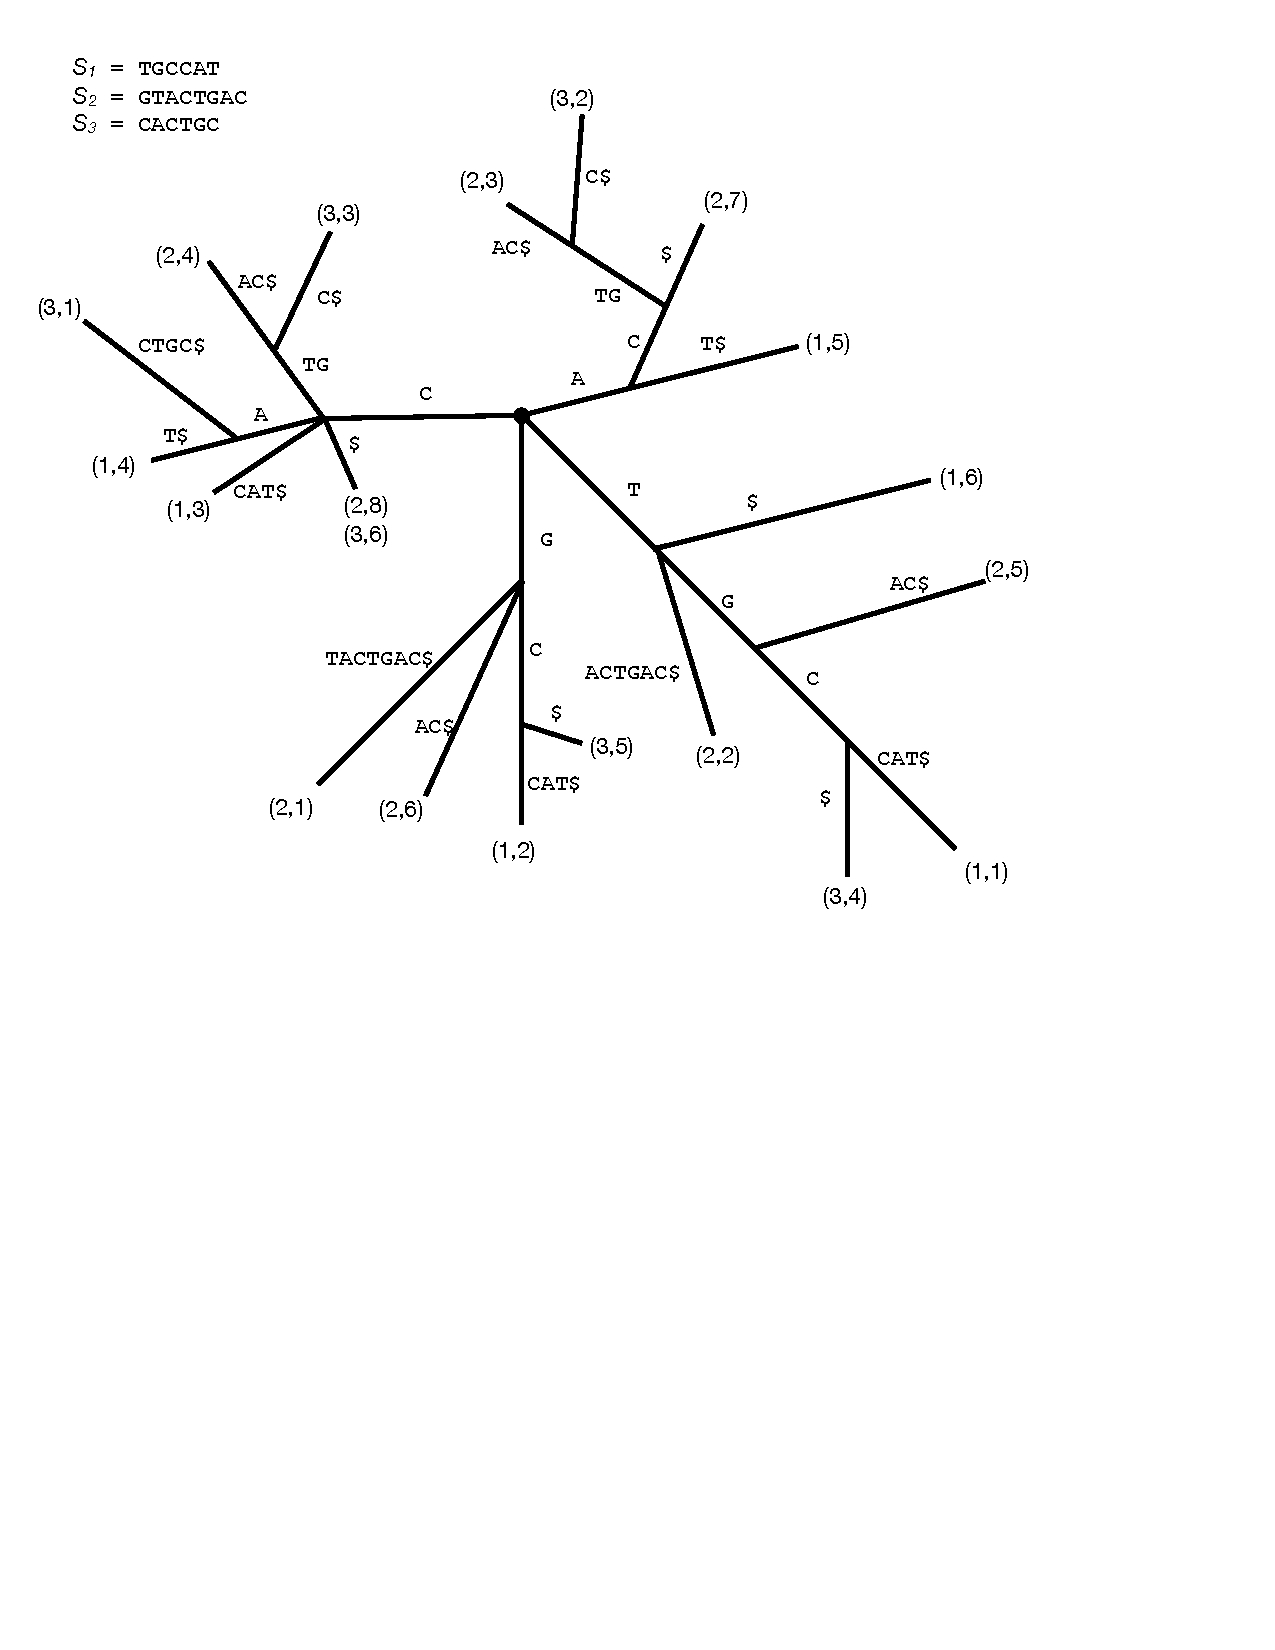
\includegraphics[width=0.7\textwidth]{Midterm_Practice_4}
\end{center}

%%%%%%%%%%%%%%%%%%%%%%%%%%%%
\clearpage
\item What is the sum-of-pairs score of the following multiple sequence alignment using the global scoring with affine scoring model with the following parameters: 
\begin{center}
\begin{tabular}{|l|l|}
\hline
match & 10\\
\hline
mismatch & -3\\
\hline
indel & -1\\
\hline
gap & -3\\
\hline
\end{tabular} \\
\vspace{3em}
\texttt{ACCTGCC}\\
\texttt{-C-TGCA}\\
\texttt{AGCGGCA}\\
\texttt{ACCT--A}\\

\end{center}
 
%%%%%%%%%%%%%%%%%%%%%%%%%%%%
\clearpage
\item Given the pairwise alignments between the 4 sequences, and using sequence $B$ as the star-center, create the multiple alignment using the center-star method. \\
\begin{center}
\begin{tabular}{|c|c|c|}
\hline
\makecell{$A$: \texttt{GATG-TGCCG} \\
$B$: \texttt{CCTGCTGCAG}}&

\makecell{$B$: \texttt{CCTGCT-GCAG}\\
$C$: \texttt{CC-GCTAGCAG} } &


\makecell{$B$: \texttt{CCTGCT-GCAG}\\
$D$: \texttt{CCTG-TAG--G}}\\
\hline
\end{tabular}
\end{center}

%%%%%%%%%%%%%%%%%%%%%%%%%%%%
\clearpage
\item How would we modify the Smith-Waterman algorithm if we wanted to find a disjoint set of substrings of $S$ to align to a substring of $T$.

For example when aligning $S=$\texttt{GG{\color{red}AGC}GG{\color{blue}CTT}GG} with $T=$\texttt{AAAACCTTTT}, an optimal alignment would align $S[3..5]\cdot S[8..10]$ to $T[3...8]$:
\begin{center}
\texttt{{\color{red}AGC}{\color{blue}CTT}}\\
\texttt{AACCTT}.
\end{center}
The concept can be though of as ``skipping'' $S[6..7]$ when computing the optimal local alignment. 
Note that the $\cdot$ operator is for concatenation. 


%%%%%%%%%%%%%%%%%%%%%%%%%%%%
 \clearpage
 \item (2 point) Given the following partially completed computation of the Z-value algorithm, compute the rest of the values using the $O(n)$ time algorithm we discussed in class.
Describe how you arrived at each value. 
\vspace{3em}
\noindent
\begin{center}
\begin{tabular}{c||c|c|c|c|c|c|c|c|c|c|c|c|c|c|c|c|c|c|}
& \texttt{C} &  \texttt{G} &  \texttt{T} &  \texttt{C} &  \texttt{G} &  \texttt{T} &  \texttt{A} &  \texttt{C} &  \texttt{G} &  \texttt{T} &  \texttt{C} &  \texttt{G} &  \texttt{A} &  \texttt{C}
\\
\hline
$i$ & 1 & 2 & 3 & 4 & 5 & 6 & 7 & 8 & 9 & 10 & 11 & 12 & 13 & 14\\
\hline
 & & & & & & & & & & & & & &\\
$Z_i$ &\Huge - & \Huge 0 & \Huge 0 & \Huge 3 & \Huge 0 & \Huge 0 & \Huge 0 & \Huge 5 & \Huge ~ ~ & \Huge ~ ~ & \Huge ~ ~ & \Huge ~ ~ & \Huge ~ ~ & \Huge ~ ~ \\
 & & & & & & & & & & & & & &\\
\hline
\end{tabular}
\end{center}

%%%%%%%%%%%%%%%%%%%%%%%%%%%%
 \clearpage
 \item (3 points) From the suffix tree below: 
(a) determine if the string \texttt{ACTG} is in the input set of sequences, and explain your reasoning;  
(b) find the longest substring that occurs in all of the sequences \textbf{\textit{twice}}, and explain your reasoning;
(c) list the missing suffix links. 
\begin{center}
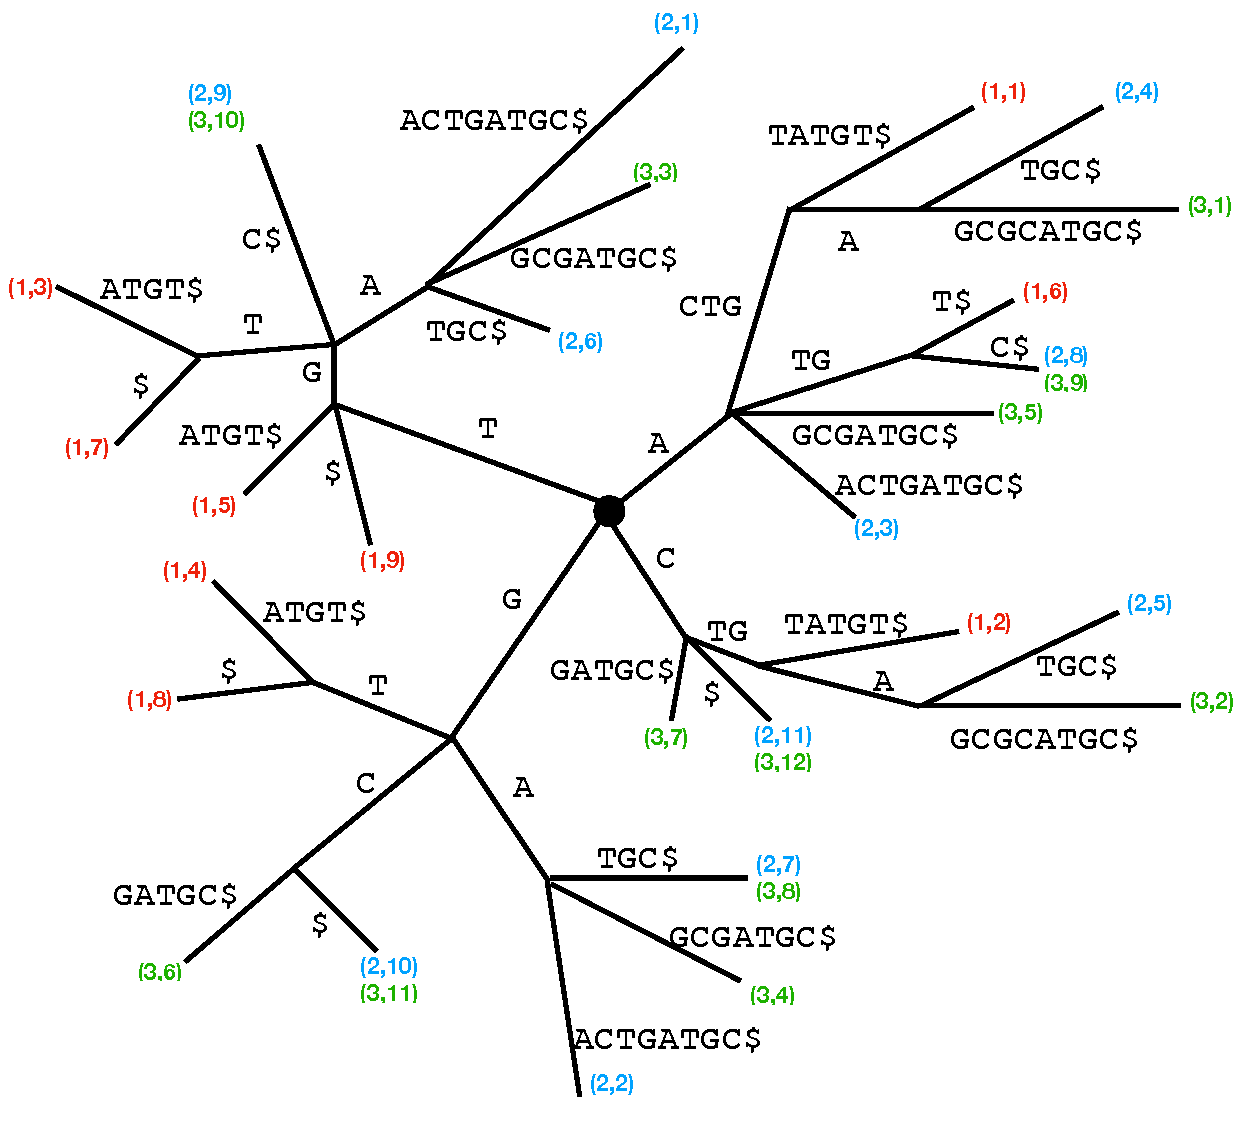
\includegraphics[width=0.85\textwidth]{Midterm_4}
\end{center}


%%%%%%%%%%%%%%%%%%%%%%%%%%%%
\clearpage
\item (2 points) How would we modify the Needleman-Wunsch algorithm if we wanted to allow for any character in $S$ to be repeated aligned as many times as we want in place.

For example when aligning $S=$\texttt{AGA} with $T=$\texttt{GGGGGA}, an optimal alignment would repeat the \texttt{G} in $S$ $5$ times to give the alignment:
\begin{center}
\texttt{AG{\color{gray!60}GGGG}A}\\
\texttt{-GGGGGA}
\end{center}
In reality, the middle \texttt{G} is is being aligned with all of the \texttt{G}s in $T$.

\end{enumerate}

\end{document}  